% adapted from https://github.com/dev-gb/TikZ-osi-model
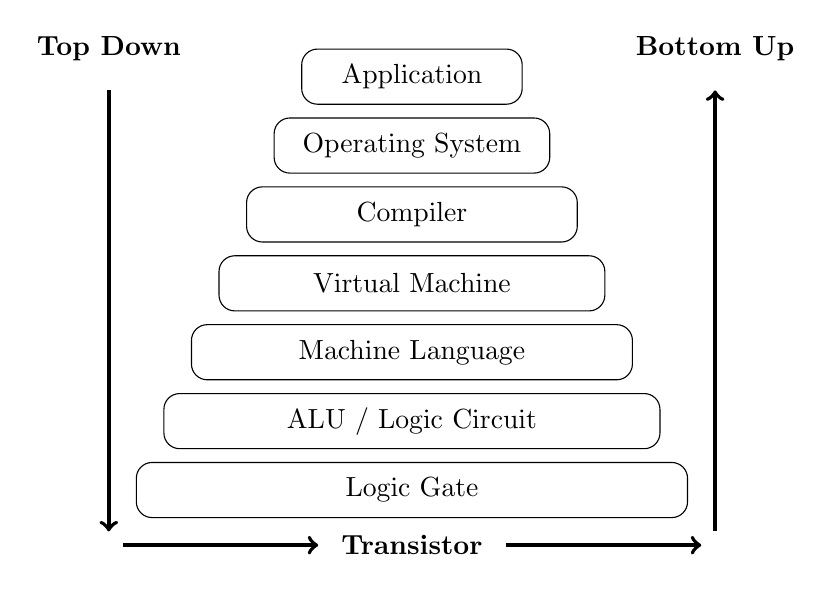
\begin{tikzpicture}[scale=0.7]

\draw[rounded corners=2mm] (-2,0) rectangle (2,-1);
\draw[rounded corners=2mm] (-2.5,-1.25) rectangle (2.5,-2.25);
\draw[rounded corners=2mm] (-3,-2.5) rectangle (3,-3.5);
\draw[rounded corners=2mm] (-3.5,-3.75) rectangle (3.5,-4.75);
\draw[rounded corners=2mm] (-4,-5) rectangle (4,-6);
\draw[rounded corners=2mm] (-4.5,-6.25) rectangle (4.5,-7.25);
\draw[rounded corners=2mm] (-5,-7.5) rectangle (5,-8.5);

\node at (0, -0.5) {Application};
\node at (0, -1.75) {Operating System};
\node at (0, -3) {Compiler};
\node at (0, -4.25) {Virtual Machine};
\node at (0, -5.5) {Machine Language};
\node at (0, -6.75) {\acs{ALU} / Logic Circuit};
\node at (0, -8) {Logic Gate};

\node[align = center] at (-5.5, 0) {\textbf{Top Down}};
\node[align = center] at (5.5, 0) {\textbf{Bottom Up}};
\node at (0, -9) {\textbf{Transistor}};

\draw[->, line width=0.5mm] (-5.5,-0.75) -- (-5.5,-8.75);
\draw[->, line width=0.5mm] (-5.25,-9) -- (-1.7,-9);
\draw[->, line width=0.5mm] (1.7,-9) -- (5.25,-9);
\draw[->, line width=0.5mm] (5.5,-8.75) -- (5.5,-0.75);

\end{tikzpicture}
